\documentclass[pdf]{beamer}

\usepackage{graphicx}
\usepackage[dvipsnames]{xcolor}
\usepackage{subfig}

\mode<presentation>{}

\usetheme{Rochester}

\setbeamertemplate{caption}{\insertcaption}
\captionsetup[subfloat]{labelformat=empty}


\title{A good programming language is a \textit{Functional} one}
\author{Artin Ghasivand}

\newcommand{\code}[1]{\textcolor{Orange}{\textsf{#1}}}

\begin{document}

\begin{frame}
  \titlepage
\end{frame}

\section{Models of Computation}
\label{sec:models-of-computation}

\begin{frame}{People}
  \begin{figure}[ht!]
    \centering
    \subfloat[Alonzo Church, Lambda-Calculus]{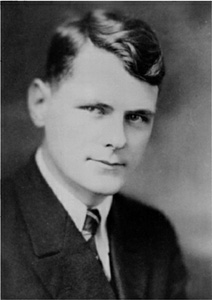
\includegraphics[width=0.30\linewidth]{Alonzo-Church}}
    \hspace{0.1cm}
    \subfloat[Kurt Gödel, Recursive Functions]{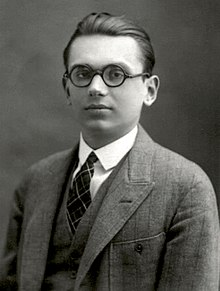
\includegraphics[width=0.30\linewidth]{Kurt-Godel}}
    \hspace{0.1cm}
    \subfloat[Alan Turing, Turing Machine]{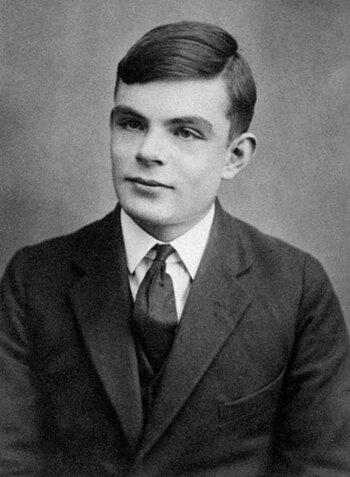
\includegraphics[width=0.30\linewidth]{Alan-Turing}}
  \end{figure}
\end{frame}

\begin{frame}

\end{frame}

\section{History of Programming Languages}
\label{sec:history}

\section{Functional Programming}
\label{sec:fp}

\begin{frame}{Some Functional Languages}
  \begin{itemize}
  \item Haskell
  \item Idris2
  \item Lean4
  \item OCaml
  \item Emacs Lisp
  \item Racket
  \item Common Lisp
  \item Scheme
  \item Clojure
  \item Erlang
  \item Gleam
  \item Standard ML
  \item Scala
  \item Elixir
  \item OCaml
  \item F\#
  \item Miranda
  \end{itemize}
\end{frame}

\begin{frame}{Lisp}
  \begin{figure}[H]
    \centering
    \subfloat[John McCarthy]{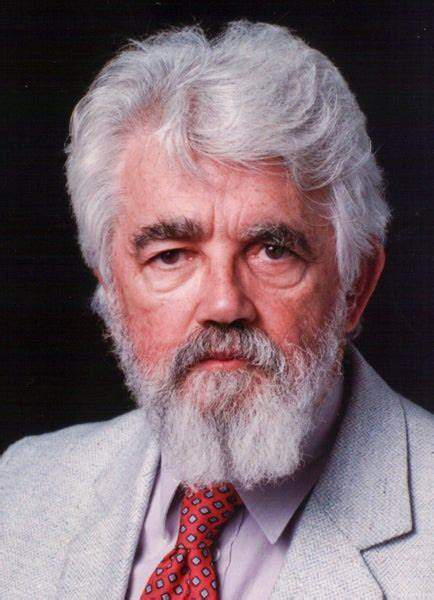
\includegraphics[width=0.33\textwidth]{John-McCarthy}}
    \hspace{0.3cm}
    \subfloat[Lisp]{
\includegraphics[width=0.33\textwidth]{LISP}}
  \end{figure}
  Short for \textit{List Processing}, Lisp is a family of \textit{Meta-programming} languages based on the \textit{Untyped Lambda-Calculus} first specified by John McCarthy.


\end{frame}
\begin{frame}{Lisp}
  \begin{figure}[H]
    \centering
    
\includegraphics[width=0.33\textwidth]{LISP}
  \end{figure}
  Inventions of Lisp:
  \begin{itemize}
  \item Garbage collection
  \item Read-Eval-Print Loop, i.e. REPL
  \item Dynamic Typing
  \item Conditionals
  \item Higher-Order functions
  \item Recursion
  \end{itemize}
\end{frame}

\begin{frame}{Miranda}
  \begin{figure}[H]
    \centering
    \subfloat[David Turner]{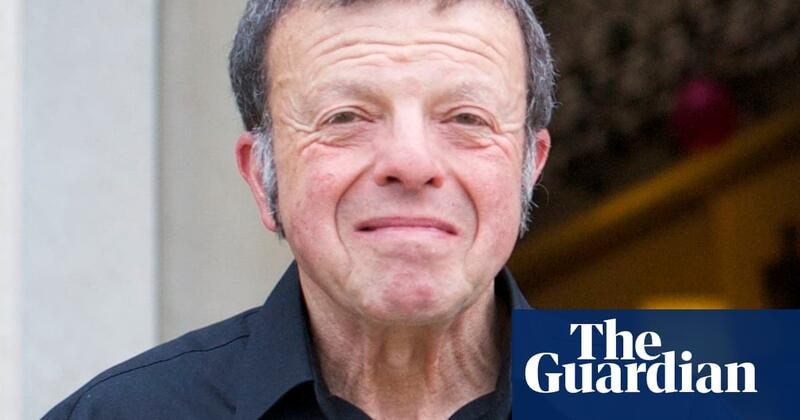
\includegraphics[width=0.40\linewidth]{David-Turner}}
    \hspace{0.3cm}
    \subfloat[Miranda]{
\includegraphics[width=0.33\linewidth]{Miranda}}
  \end{figure}
\end{frame}

\begin{frame}{Haskell}
  \begin{figure}[H]
    \centering
    \subfloat[Working group 2.8]{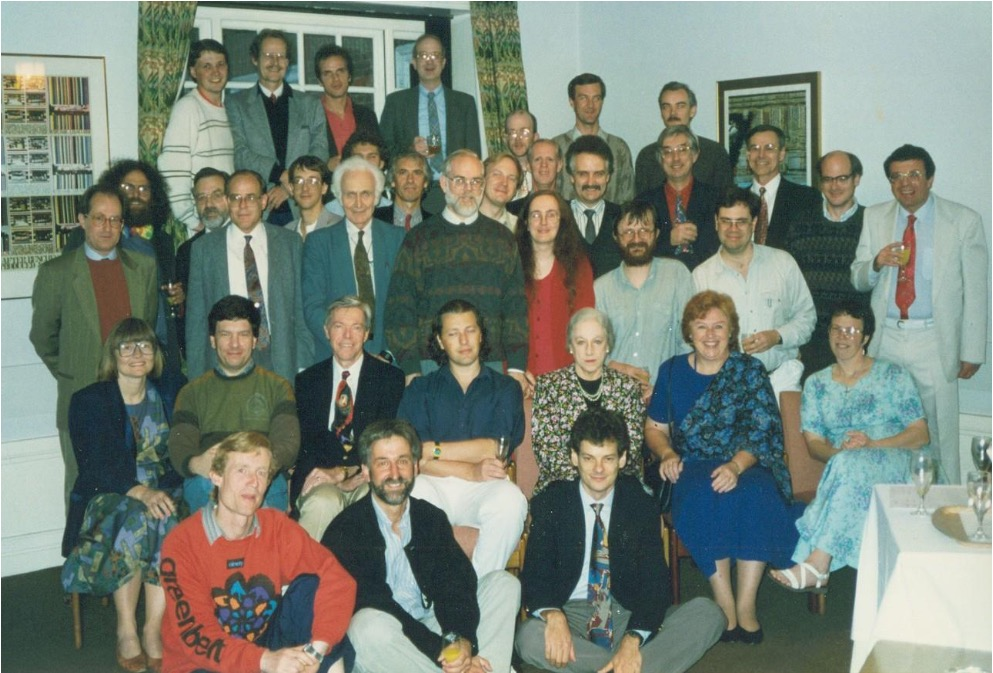
\includegraphics[width=0.33\textwidth]{haskell-working-group}}
    \hspace{0.3cm}
    \subfloat[Haskell]{
\includegraphics[width=0.33\textwidth]{haskell-logo}}
  \end{figure}
\end{frame}

\begin{frame}{Haskell}
  Some of the features:
  \begin{itemize}
  \item Referential Transparency
  \item Purity
  \item Laziness
  \item Type Classes (ad-hoc polymorphism)
  \item Type Inference
  \item Impredicative Instantiation
  \item Generalized Algebraic Datatypes
  \item Existential Types
  \item Type Families
  \item Guards
  \item Type Abstractions
  \item Higher-Rank Types
  \item Kind Polymorphism
  \item Dependent Kinds
  \end{itemize}

\end{frame}

\begin{frame}{The love for operators}

  Haskellers love operators. They let us convey algebraic laws easier than with functions

\end{frame}

\begin{frame}{Data Constructors and Patterns}
  The same tools that let me put some \textit{data} together allows us to take it apart.
  TODO Talk about data constructors and pattern matching
\end{frame}

\begin{frame}
  Lazy Evaluation, is an evaluation model where things get evaluated only when they \textit{need} to.

  Benefits of Laziness: (TODO Find more stuff)
  \begin{itemize}
  \item Infinite data structures
  \item Defining control-flow as functions instead of primitives or macros
  \item Lazy programs tend to terminate more than strict ones (TODO Double check)
  \item \textit{Forces} purity (TODO This may be unrelated and maybe you should just remove it)
  \end{itemize}
\end{frame}

\section{Types}
\label{sec:types}

\begin{frame}[fragile]{Type Inference}
\begin{verbatim}
and True x  = x
and False _ = False
\end{verbatim}

  Haskell is smart enough to \textit{infer} the type of \code{and}:

  \code{Bool $\to$ Bool $\to$ Bool}

  By itself, and if you give it the wrong argument, it will tell you exactly what you did wrong!

  e.g. \verb|test = and True 'c'| will result in the following error message:
  \begin{figure}[H]
    \centering
    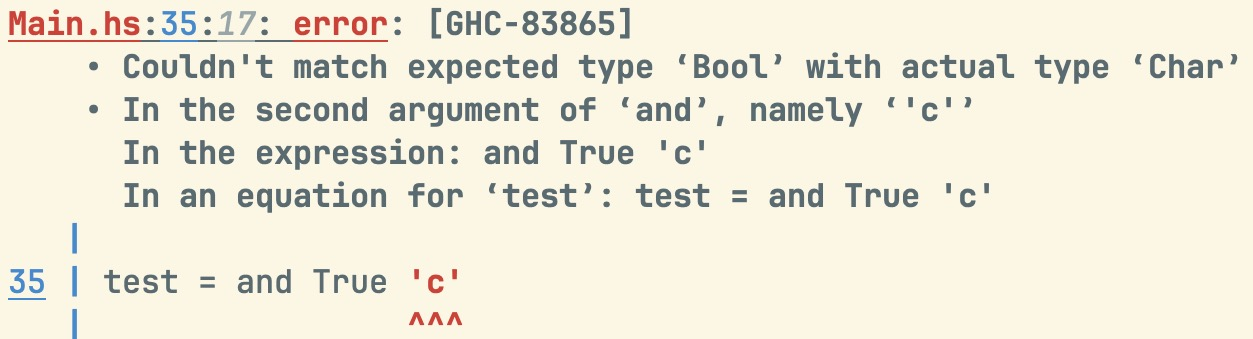
\includegraphics[width=\linewidth]{and-type-error}
  \end{figure}
\end{frame}



\section{Pure and Lazy Functional Programming}
\label{sec:pure-lazy-fp}

\begin{frame}[fragile]{Example: \code{factorial} in Python}
  \begin{figure}[H]
    \centering
    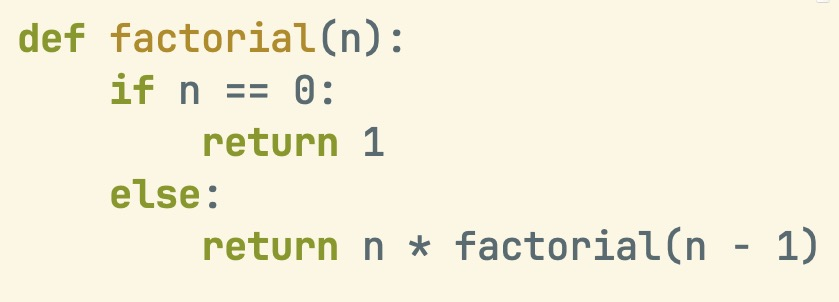
\includegraphics[width=\linewidth]{factorial-py}
  \end{figure}
\end{frame}

\begin{frame}[fragile]{Example: \code{factorial} in Haskell}
    \begin{figure}[H]
    \centering
    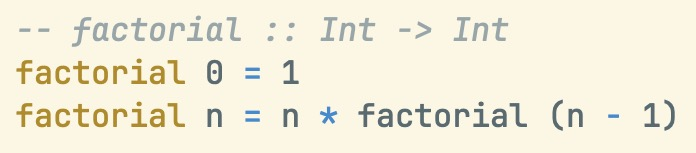
\includegraphics[width=\linewidth]{factorial-hs}
  \end{figure}

  \pause
  Let's evaluate \code{factorial 3}:

  \begin{enumerate}
    \item<1-> \code{factorial 3}
    \item<2-> \code{3 * factorial 2}
    \item<3-> \code{3 * 2 * factorial 1}
    \item<4-> \code{3 * 2 * 1 * factorial 0}
    \item<5-> \code{3 * 2 * 1 * 1}
    \item<6-> \code{6 * 1 * 1}
    \item<7-> \code{6 * 1}
    \item<8-> \code{6}
  \end{enumerate}

\end{frame}

\begin{frame}[fragile]{Example: \code{say} in Python}

  \code{say} is a function that given a number \textit{n} and a string \textit{string}, will repeat the \textit{string} \textit{n} times.

  e.g. \code{say(2,"Hi ") = "Hi Hi "}

  \begin{figure}[H]
    \centering
    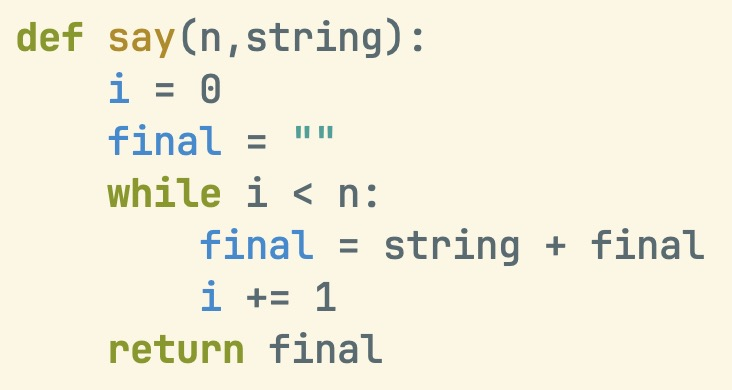
\includegraphics[width=\linewidth]{say-py}
  \end{figure}

\end{frame}

\begin{frame}[fragile]{Example: \code{say} in Haskell}
  The \code{++} operator concatenates two strings together.

  \begin{figure}[H]
    \centering
    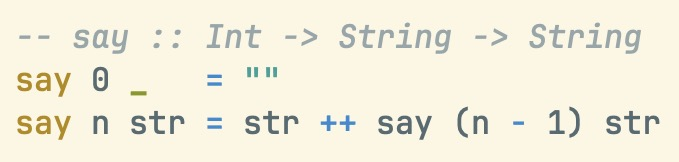
\includegraphics[width=\linewidth]{say-hs}
  \end{figure}

  \pause
  Let's evaluate \code{say 2 "Hi "}:

  \begin{enumerate}
    \item<1-> \code{say 2 "Hi "}
    \item<2-> \code{"Hi " ++ say 1 "Hi"}
    \item<3-> \code{"Hi " ++ "Hi " ++ say 0 "Hi"}
    \item<4-> \code{"Hi " ++ "Hi " ++ ""}
    \item<5-> \code{"Hi Hi " ++ ""}
    \item<6-> \code{"Hi Hi "}
  \end{enumerate}

\end{frame}

\begin{frame}[fragile]{Example: \code{hasEven} in Python}
  \code{hasEven} is a function that given a character, \textit{char}
  ,and a string \textit{string}, will return \textit{true} if the number
  of times \textit{char} occurs in \textit{string} is even.

  \begin{figure}[H]
    \centering
    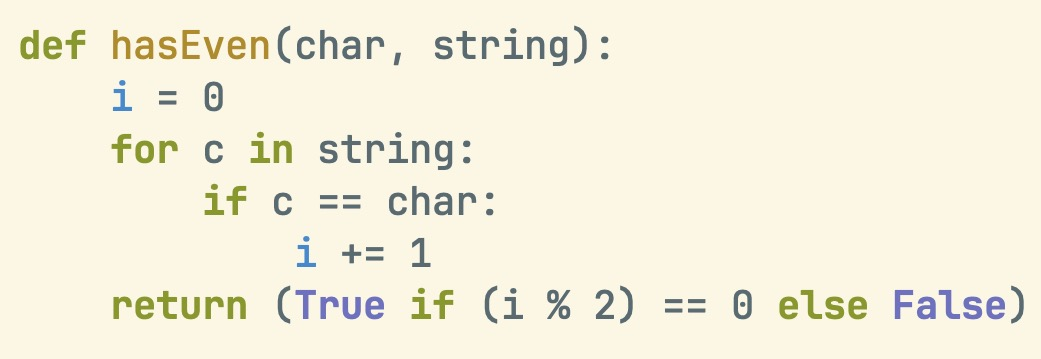
\includegraphics[width=\linewidth]{hasEven-py}
  \end{figure}

\end{frame}

\begin{frame}{Example: \code{hasEven} in Haskell}
  \code{even} is a built-in function that says whether its input is even or not.
    \begin{figure}[H]
    \centering
    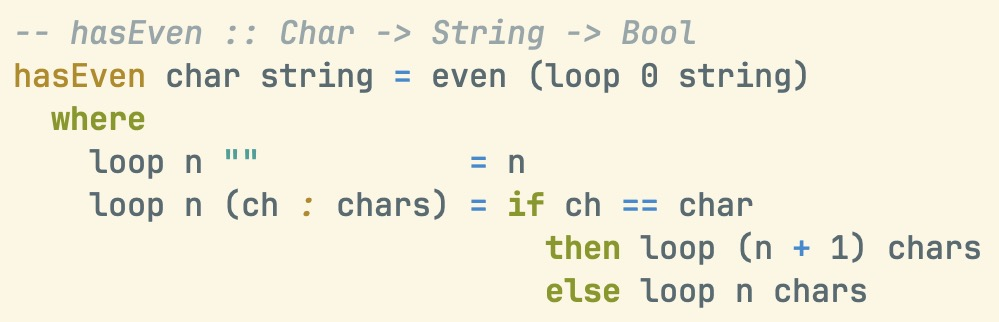
\includegraphics[width=\linewidth]{hasEven-hs}
  \end{figure}
\end{frame}

\begin{frame}{Example: \code{hasEven} in Haskell}
    \begin{figure}[H]
    \centering
    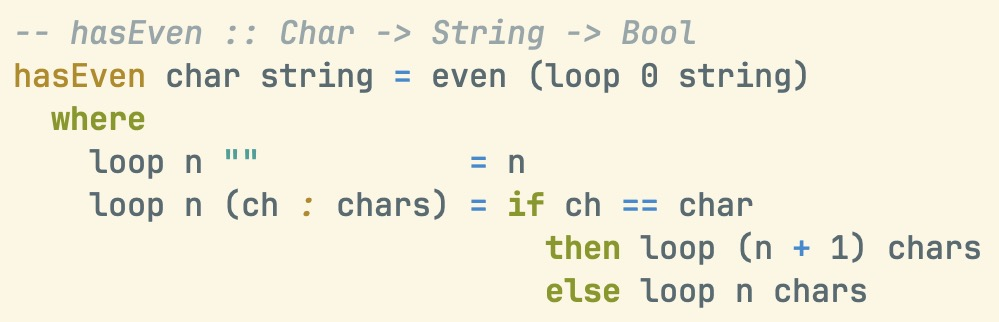
\includegraphics[width=0.80\linewidth]{hasEven-hs}
  \end{figure}

  \pause
  Let's evaluate \code{hasEven 'e' "eyes"}:

  \begin{enumerate}
    \item<1-> \code{even (loop 0 "eyes")}
    \item<2-> \code{even (loop 1 "yes")}
    \item<3-> \code{even (loop 1 "es")}
    \item<4-> \code{even (loop 2 "s")}
    \item<5-> \code{even (loop 2 "")}
    \item<6-> \code{even 2}
    \item<7-> \code{True}
  \end{enumerate}

\end{frame}

\section{Influence of functional languages on imperative languages}
\label{sec:influence}

\section{Learning more}
\label{sec:learning-more}

\end{document}
